\documentclass[../ComplexAnalysis_Notes.tex]{subfiles}
\myexternaldocument{./lec-04}

\begin{document}
\chapter*{Lecture 5} %Set chapter name
\addcontentsline{toc}{chapter}{Lecture 5} %Set chapter title
\setcounter{chapter}{5} %Set chapter counter
\setcounter{section}{0}
\setcounter{equation}{0}
\setcounter{figure}{0}

Before developing some more tools required to prove the Cauchy-Goursat theorem, we give some more motivation towards the result; what happens for \( C^1 \) functions. Recall Stokes's theorem for \( \mathbbm{R}^2 \): Consider a simply connected region \( \Omega \subseteq \mathbbm{R}^2 \) with piecewise smooth, simple and closed boundary \( \partial \Omega \). If \( f = P \dd{x} + Q \dd{y} \) is a \( C^1 \) \( 1- \)form on an open set \( U \supseteq \Omega \cup \partial \Omega  \), then
\[ 
 \oint_{\partial \Omega} f = \iint_{\Omega}\dd{f}.
 \]
Now, as \( f = P \dd{x} + Q \dd{y} \), we get \( \dd{f} = \dd{P} \dd{x} + \dd{Q} \dd{y} = P_y \dd{y}\dd{x} + Q_x \dd{x}\dd{y} = (Q_x-P_y)\dd{x}\dd{y} \). Hence,
\[ 
  \oint_{\partial \Omega} f = \oint_{\partial \Omega} P \dd{x} + Q \dd{y} = \iint_\Omega \qty(\pdv{Q}{x} - \pdv{P}{y}) \dd{x} \dd{y}
 \]
which is nothing but the statement of Green's theorem. We now return to \( \mathbbm{C} \) and assume \( f \in \textsf{Hol}(\Omega) \cap C^1(\Omega) \), where \( \Omega \) is a simply connected region as above. Let \( \gamma \subseteq \Omega \) be a piecewise smooth, simple and closed curve. Then, by the discussion of lecture 3,
\[ 
 \oint_\gamma f \dd{z} = \qty(\oint_\gamma u \dd{x} - v \dd{y}) + i\qty(\oint_\gamma v \dd{x} + u \dd{y}) 
 \]
 Using Stokes's theorem on the two integrals on the right we get,
 \[ 
  \oint_\gamma f \dd{z} = \iint_{\Sigma \gamma} \qty(-\pdv{v}{x}-\pdv{u}{y})\dd{x}\dd{y} + i \iint_{\Sigma \gamma} \qty(\pdv{u}{x}-\pdv{v}{y})\dd{x}\dd{y} = 0
  \]
  where the final equality follows from the Cauchy-Riemann equations. This is exactly the statement of the Cauchy-Goursat theorem! We now set to develop the tools needed to remove the \( C^1 \) restriction, that is, to show that holomorphic functions must be \( C^1 \) on ``nice'' domains.

\textbf{Exercise}: Suppose \( f \in C^1(\Omega) \), where \( \Omega \) is as above. If \( \gamma \) is a curve as above, show that
\[ 
 \oint_\gamma f \dd{z} = 2 \iint_{\Sigma \gamma} \overline{\partial}f \dd{x}\dd{y}
 \]
holds for all such functions, without assuming holomorphicity.
\medskip

Recall the result from lecture 3 that
\[ 
 \frac{1}{2\pi i} \oint_{C_r(0)} \frac{1}{z} = 1
 \]
 for any \( r > 0 \). Changing variables, we get the equality
 \[ 
  \frac{1}{2\pi i} \oint_{C_r(z_0)} \frac{1}{z-z_0} = 1
  \]
for any \( z_0 \in \mathbbm{C} \). We now generalise this result to the following very useful theorem.

\begin{Thm}{Cauchy Integral Formula}{cauchy_formula}
 \, Let \( f \in \textsf{Hol}(\mathcal{O}) \) and \( C \subseteq \mathcal{O} \) be a circle such that \( D = C \cup \Sigma C \) is in \( \mathcal{O} \). Then, for all \( z \in \Sigma C \),
 \[ 
  \frac{1}{2\pi i} \oint_C \frac{f(\zeta)}{\zeta-z}\dd{\zeta} = f(z).
  \]
 \end{Thm}

\textbf{Remark}: Note that if \( z \in \mathcal{O} \setminus D \), by Theorem \ref{thm:4.2},
\[ 
  \frac{1}{2\pi i} \oint_C \frac{f(\zeta)}{\zeta-z}\dd{\zeta} = 0.
 \]

\begin{wrapfigure}{r}{0mm}
\centering 
\tikzset{every picture/.style={line width=0.75pt}} %set default line width to 0.75pt        

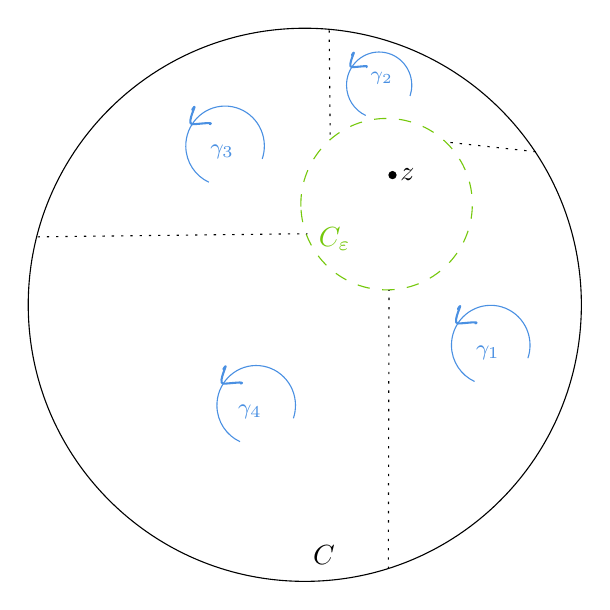
\begin{tikzpicture}[x=0.75pt,y=0.75pt,yscale=-1,xscale=1][thbp]
%uncomment if require: \path (0,535); %set diagram left start at 0, and has height of 535

%Shape: Circle [id:dp07184970632773247] 
\draw  [color={rgb, 255:red, 117; green, 200; blue, 12 }  ,draw opacity=1 ][dash pattern={on 4.5pt off 4.5pt}] (276.86,191.92) .. controls (276.22,169.12) and (294.19,150.11) .. (317,149.47) .. controls (339.8,148.83) and (358.81,166.79) .. (359.45,189.6) .. controls (360.09,212.41) and (342.12,231.41) .. (319.32,232.05) .. controls (296.51,232.69) and (277.5,214.73) .. (276.86,191.92) -- cycle ;
%Shape: Circle [id:dp05798669283304125] 
\draw   (145.5,239.25) .. controls (145.5,165.66) and (205.16,106) .. (278.75,106) .. controls (352.34,106) and (412,165.66) .. (412,239.25) .. controls (412,312.84) and (352.34,372.5) .. (278.75,372.5) .. controls (205.16,372.5) and (145.5,312.84) .. (145.5,239.25) -- cycle ;
%Straight Lines [id:da6079137096691299] 
\draw  [dash pattern={on 0.84pt off 2.51pt}]  (150,206.5) -- (280,205) ;
%Straight Lines [id:da3642748238679152] 
\draw  [dash pattern={on 0.84pt off 2.51pt}]  (390,165.5) -- (346,160.75) ;
%Straight Lines [id:da47429886601718296] 
\draw  [dash pattern={on 0.84pt off 2.51pt}]  (319,366.5) -- (319.32,232.05) ;
%Straight Lines [id:da35469723533772646] 
\draw  [dash pattern={on 0.84pt off 2.51pt}]  (290.5,107) -- (291,159.25) ;
%Shape: Free Drawing [id:dp10308850537066128] 
\draw  [line width=3] [line join = round][line cap = round] (321,176.75) .. controls (321,176.75) and (321,176.75) .. (321,176.75) ;
%Shape: Arc [id:dp8067887792295754] 
\draw  [draw opacity=0] (247.53,305.19) .. controls (241.06,302.22) and (236.51,295.64) .. (236.41,287.95) .. controls (236.27,277.35) and (244.62,268.64) .. (255.07,268.5) .. controls (265.53,268.36) and (274.12,276.84) .. (274.26,287.45) .. controls (274.29,289.72) and (273.93,291.91) .. (273.24,293.95) -- (255.33,287.7) -- cycle ; \draw  [color={rgb, 255:red, 74; green, 144; blue, 226 }  ,draw opacity=1 ] (247.53,305.19) .. controls (241.06,302.22) and (236.51,295.64) .. (236.41,287.95) .. controls (236.27,277.35) and (244.62,268.64) .. (255.07,268.5) .. controls (265.53,268.36) and (274.12,276.84) .. (274.26,287.45) .. controls (274.29,289.72) and (273.93,291.91) .. (273.24,293.95) ;  
%Shape: Free Drawing [id:dp05798054402708985] 
\draw  [color={rgb, 255:red, 74; green, 144; blue, 226 }  ,draw opacity=1 ][line width=0.75] [line join = round][line cap = round] (239.5,270.25) .. controls (243.28,264.57) and (236.15,277.25) .. (239.5,277.25) .. controls (242.33,277.25) and (250.53,275.98) .. (248,277.25) ;
%Shape: Arc [id:dp7052662385836276] 
\draw  [draw opacity=0] (360.53,276.19) .. controls (354.06,273.22) and (349.51,266.64) .. (349.41,258.95) .. controls (349.27,248.35) and (357.62,239.64) .. (368.07,239.5) .. controls (378.53,239.36) and (387.12,247.84) .. (387.26,258.45) .. controls (387.29,260.72) and (386.93,262.91) .. (386.24,264.95) -- (368.33,258.7) -- cycle ; \draw  [color={rgb, 255:red, 74; green, 144; blue, 226 }  ,draw opacity=1 ] (360.53,276.19) .. controls (354.06,273.22) and (349.51,266.64) .. (349.41,258.95) .. controls (349.27,248.35) and (357.62,239.64) .. (368.07,239.5) .. controls (378.53,239.36) and (387.12,247.84) .. (387.26,258.45) .. controls (387.29,260.72) and (386.93,262.91) .. (386.24,264.95) ;  
%Shape: Free Drawing [id:dp9189156294889053] 
\draw  [color={rgb, 255:red, 74; green, 144; blue, 226 }  ,draw opacity=1 ][line width=0.75] [line join = round][line cap = round] (352.5,241.25) .. controls (356.28,235.57) and (349.15,248.25) .. (352.5,248.25) .. controls (355.33,248.25) and (363.53,246.98) .. (361,248.25) ;
%Shape: Arc [id:dp6344234479165585] 
\draw  [draw opacity=0] (308.08,148.01) .. controls (302.71,145.53) and (298.95,140.06) .. (298.86,133.66) .. controls (298.74,124.83) and (305.68,117.58) .. (314.36,117.46) .. controls (323.04,117.34) and (330.17,124.41) .. (330.29,133.24) .. controls (330.31,135.13) and (330.01,136.95) .. (329.45,138.64) -- (314.57,133.45) -- cycle ; \draw  [color={rgb, 255:red, 74; green, 144; blue, 226 }  ,draw opacity=1 ] (308.08,148.01) .. controls (302.71,145.53) and (298.95,140.06) .. (298.86,133.66) .. controls (298.74,124.83) and (305.68,117.58) .. (314.36,117.46) .. controls (323.04,117.34) and (330.17,124.41) .. (330.29,133.24) .. controls (330.31,135.13) and (330.01,136.95) .. (329.45,138.64) ;  
%Shape: Free Drawing [id:dp2392567095367938] 
\draw  [color={rgb, 255:red, 74; green, 144; blue, 226 }  ,draw opacity=1 ][line width=0.75] [line join = round][line cap = round] (301.43,118.92) .. controls (304.57,114.19) and (298.65,124.75) .. (301.43,124.75) .. controls (303.78,124.75) and (310.59,123.69) .. (308.49,124.75) ;
%Shape: Arc [id:dp3224835523886671] 
\draw  [draw opacity=0] (232.53,180.19) .. controls (226.06,177.22) and (221.51,170.64) .. (221.41,162.95) .. controls (221.27,152.35) and (229.62,143.64) .. (240.07,143.5) .. controls (250.53,143.36) and (259.12,151.84) .. (259.26,162.45) .. controls (259.29,164.72) and (258.93,166.91) .. (258.24,168.95) -- (240.33,162.7) -- cycle ; \draw  [color={rgb, 255:red, 74; green, 144; blue, 226 }  ,draw opacity=1 ] (232.53,180.19) .. controls (226.06,177.22) and (221.51,170.64) .. (221.41,162.95) .. controls (221.27,152.35) and (229.62,143.64) .. (240.07,143.5) .. controls (250.53,143.36) and (259.12,151.84) .. (259.26,162.45) .. controls (259.29,164.72) and (258.93,166.91) .. (258.24,168.95) ;  
%Shape: Free Drawing [id:dp9016204510340234] 
\draw  [color={rgb, 255:red, 74; green, 144; blue, 226 }  ,draw opacity=1 ][line width=0.75] [line join = round][line cap = round] (224.5,145.25) .. controls (228.28,139.57) and (221.15,152.25) .. (224.5,152.25) .. controls (227.33,152.25) and (235.53,150.98) .. (233,152.25) ;

% Text Node
\draw (323.5,172.5) node [anchor=north west][inner sep=0.75pt]   [align=left] {$\displaystyle z$};
% Text Node
\draw (257.53,290.92) node  [font=\footnotesize,color={rgb, 255:red, 74; green, 144; blue, 226 }  ,opacity=1 ] [align=left] {\begin{minipage}[lt]{16.32pt}\setlength\topsep{0pt}
$\displaystyle \gamma _{4}$
\end{minipage}};
% Text Node
\draw (372.13,262.32) node  [font=\footnotesize,color={rgb, 255:red, 74; green, 144; blue, 226 }  ,opacity=1 ] [align=left] {\begin{minipage}[lt]{16.32pt}\setlength\topsep{0pt}
$\displaystyle \gamma _{1}$
\end{minipage}};
% Text Node
\draw (319.41,130.17) node  [font=\scriptsize,color={rgb, 255:red, 74; green, 144; blue, 226 }  ,opacity=1 ] [align=left] {\begin{minipage}[lt]{13.59pt}\setlength\topsep{0pt}
$\displaystyle {\textstyle \gamma _{2}}$
\end{minipage}};
% Text Node
\draw (244.13,165.52) node  [font=\footnotesize,color={rgb, 255:red, 74; green, 144; blue, 226 }  ,opacity=1 ] [align=left] {\begin{minipage}[lt]{16.32pt}\setlength\topsep{0pt}
$\displaystyle \gamma _{3}$
\end{minipage}};
% Text Node
\draw (289.8,359.95) node   [align=left] {\begin{minipage}[lt]{10.61pt}\setlength\topsep{0pt}
$\displaystyle C$
\end{minipage}};
% Text Node
\draw (292.6,207.55) node  [color={rgb, 255:red, 117; green, 200; blue, 12 }  ,opacity=1 ] [align=left] {\begin{minipage}[lt]{10.61pt}\setlength\topsep{0pt}
$\displaystyle C_{\varepsilon }$
\end{minipage}};


  \end{tikzpicture}

\end{wrapfigure}
 

\begin{proof} 
  Fix \( z \in \Sigma C \) and let \( B_\varepsilon (z) \subseteq \Sigma C \), \( C_\varepsilon = \partial B_\varepsilon(z) \). We claim,
  \[ 
   \oint_C \frac{f(\zeta)}{\zeta-z} \dd{\zeta} = \oint_{C_\varepsilon} \frac{f(\zeta)}{\zeta-z} \dd{\zeta}
   \]
Introduce 4 ``cuts'' as shown by the dotted lines in the figure, and let the loops displayed be oriented anticlockwise. Then, \( \gamma_1 \cup \gamma_2 \cup \gamma_3 \cup \gamma_4 = C  \cup (-C_\varepsilon) \). Further, 
\[ 
 \zeta \mapsto \frac{f(\zeta)}{\zeta-z} 
 \]
is holomorphic in \( \Sigma \gamma_j \) for each \( j \). As each of these sets \( \Sigma \gamma_j \) can be covered by an open convex set \( \Omega_j \subseteq \mathcal{O} \), we get by Theorem \ref{thm:4.2} that
\[ 
 \oint_{\gamma_j} \frac{f(\zeta)}{\zeta-z} \dd{\zeta}= 0
 \]
for each \( j \). Therefore, as integration over \( \cup \gamma_j \) is simply the sum of each of these integrals, we get
\begin{align*}
   \oint_C \frac{f(\zeta)}{\zeta-z} \dd{\zeta} 
   &= \oint_{C_\varepsilon} \frac{f(\zeta)}{\zeta-z} \dd{\zeta} \\
   \implies \frac{1}{2\pi i}\oint_C \frac{f(\zeta)}{\zeta-z} \dd{\zeta} -f(z)
   &= \frac{1}{2\pi i}\oint_{C_\varepsilon} \frac{f(\zeta)}{\zeta-z} \dd{\zeta} 
   - \frac{f(z)}{2\pi i}\oint_{C_\varepsilon} \frac{1}{\zeta-z} \dd{\zeta} \\
   \implies \frac{1}{2\pi i}\oint_C \frac{f(\zeta)}{\zeta-z} \dd{\zeta} -f(z)
   &= \frac{1}{2\pi i}\oint_{C_\varepsilon} \frac{f(\zeta)-f(z)}{\zeta-z} \dd{\zeta}
\end{align*}
By the triangle inequality,
\[ 
  \abs{\frac{1}{2\pi i}\oint_{C_\varepsilon} \frac{f(\zeta)-f(z)}{\zeta-z} \dd{\zeta}} \leq \frac{1}{2\pi} \sup_{\zeta \in C_\varepsilon} \abs{\frac{f(\zeta)-f(z)}{\zeta-z}} \ell(C_\varepsilon) = \varepsilon \sup_{\zeta \in C_\varepsilon} \abs{\frac{f(\zeta)-f(z)}{\zeta-z}}
 \]
As \( \varepsilon \to 0 \), the supremum goes to \( \abs{f'(z)} \) and so the right most quantity goes to 0. Therefore, in light of the equality above, we get
\[ 
  \frac{1}{2\pi i}\oint_C \frac{f(\zeta)}{\zeta-z} \dd{\zeta} -f(z) = 0
 \]
 as was to be shown.
\end{proof}
\end{document}